% Options for packages loaded elsewhere
\PassOptionsToPackage{unicode}{hyperref}
\PassOptionsToPackage{hyphens}{url}
\PassOptionsToPackage{dvipsnames,svgnames,x11names}{xcolor}
%
\documentclass[
  singlecolumn,
  9pt]{report}

\usepackage{amsmath,amssymb}
\usepackage{iftex}
\ifPDFTeX
  \usepackage[T1]{fontenc}
  \usepackage[utf8]{inputenc}
  \usepackage{textcomp} % provide euro and other symbols
\else % if luatex or xetex
  \usepackage{unicode-math}
  \defaultfontfeatures{Scale=MatchLowercase}
  \defaultfontfeatures[\rmfamily]{Ligatures=TeX,Scale=1}
\fi
\usepackage[]{libertinus}
\ifPDFTeX\else  
    % xetex/luatex font selection
\fi
% Use upquote if available, for straight quotes in verbatim environments
\IfFileExists{upquote.sty}{\usepackage{upquote}}{}
\IfFileExists{microtype.sty}{% use microtype if available
  \usepackage[]{microtype}
  \UseMicrotypeSet[protrusion]{basicmath} % disable protrusion for tt fonts
}{}
\makeatletter
\@ifundefined{KOMAClassName}{% if non-KOMA class
  \IfFileExists{parskip.sty}{%
    \usepackage{parskip}
  }{% else
    \setlength{\parindent}{0pt}
    \setlength{\parskip}{6pt plus 2pt minus 1pt}}
}{% if KOMA class
  \KOMAoptions{parskip=half}}
\makeatother
\usepackage{xcolor}
\usepackage[top=30mm,bottom=30mm,left=20mm,heightrounded]{geometry}
\setlength{\emergencystretch}{3em} % prevent overfull lines
\setcounter{secnumdepth}{-\maxdimen} % remove section numbering
% Make \paragraph and \subparagraph free-standing
\ifx\paragraph\undefined\else
  \let\oldparagraph\paragraph
  \renewcommand{\paragraph}[1]{\oldparagraph{#1}\mbox{}}
\fi
\ifx\subparagraph\undefined\else
  \let\oldsubparagraph\subparagraph
  \renewcommand{\subparagraph}[1]{\oldsubparagraph{#1}\mbox{}}
\fi


\providecommand{\tightlist}{%
  \setlength{\itemsep}{0pt}\setlength{\parskip}{0pt}}\usepackage{longtable,booktabs,array}
\usepackage{calc} % for calculating minipage widths
% Correct order of tables after \paragraph or \subparagraph
\usepackage{etoolbox}
\makeatletter
\patchcmd\longtable{\par}{\if@noskipsec\mbox{}\fi\par}{}{}
\makeatother
% Allow footnotes in longtable head/foot
\IfFileExists{footnotehyper.sty}{\usepackage{footnotehyper}}{\usepackage{footnote}}
\makesavenoteenv{longtable}
\usepackage{graphicx}
\makeatletter
\def\maxwidth{\ifdim\Gin@nat@width>\linewidth\linewidth\else\Gin@nat@width\fi}
\def\maxheight{\ifdim\Gin@nat@height>\textheight\textheight\else\Gin@nat@height\fi}
\makeatother
% Scale images if necessary, so that they will not overflow the page
% margins by default, and it is still possible to overwrite the defaults
% using explicit options in \includegraphics[width, height, ...]{}
\setkeys{Gin}{width=\maxwidth,height=\maxheight,keepaspectratio}
% Set default figure placement to htbp
\makeatletter
\def\fps@figure{htbp}
\makeatother
% definitions for citeproc citations
\NewDocumentCommand\citeproctext{}{}
\NewDocumentCommand\citeproc{mm}{%
  \begingroup\def\citeproctext{#2}\cite{#1}\endgroup}
\makeatletter
 % allow citations to break across lines
 \let\@cite@ofmt\@firstofone
 % avoid brackets around text for \cite:
 \def\@biblabel#1{}
 \def\@cite#1#2{{#1\if@tempswa , #2\fi}}
\makeatother
\newlength{\cslhangindent}
\setlength{\cslhangindent}{1.5em}
\newlength{\csllabelwidth}
\setlength{\csllabelwidth}{3em}
\newenvironment{CSLReferences}[2] % #1 hanging-indent, #2 entry-spacing
 {\begin{list}{}{%
  \setlength{\itemindent}{0pt}
  \setlength{\leftmargin}{0pt}
  \setlength{\parsep}{0pt}
  % turn on hanging indent if param 1 is 1
  \ifodd #1
   \setlength{\leftmargin}{\cslhangindent}
   \setlength{\itemindent}{-1\cslhangindent}
  \fi
  % set entry spacing
  \setlength{\itemsep}{#2\baselineskip}}}
 {\end{list}}
\usepackage{calc}
\newcommand{\CSLBlock}[1]{\hfill\break#1\hfill\break}
\newcommand{\CSLLeftMargin}[1]{\parbox[t]{\csllabelwidth}{\strut#1\strut}}
\newcommand{\CSLRightInline}[1]{\parbox[t]{\linewidth - \csllabelwidth}{\strut#1\strut}}
\newcommand{\CSLIndent}[1]{\hspace{\cslhangindent}#1}

\usepackage{cancel}
\usepackage[noblocks]{authblk}
\renewcommand*{\Authsep}{, }
\renewcommand*{\Authand}{, }
\renewcommand*{\Authands}{, }
\renewcommand\Affilfont{\small}
\usepackage{cancel}
\makeatletter
\@ifpackageloaded{caption}{}{\usepackage{caption}}
\AtBeginDocument{%
\ifdefined\contentsname
  \renewcommand*\contentsname{Table of contents}
\else
  \newcommand\contentsname{Table of contents}
\fi
\ifdefined\listfigurename
  \renewcommand*\listfigurename{List of Figures}
\else
  \newcommand\listfigurename{List of Figures}
\fi
\ifdefined\listtablename
  \renewcommand*\listtablename{List of Tables}
\else
  \newcommand\listtablename{List of Tables}
\fi
\ifdefined\figurename
  \renewcommand*\figurename{Figure}
\else
  \newcommand\figurename{Figure}
\fi
\ifdefined\tablename
  \renewcommand*\tablename{Table}
\else
  \newcommand\tablename{Table}
\fi
}
\@ifpackageloaded{float}{}{\usepackage{float}}
\floatstyle{ruled}
\@ifundefined{c@chapter}{\newfloat{codelisting}{h}{lop}}{\newfloat{codelisting}{h}{lop}[chapter]}
\floatname{codelisting}{Listing}
\newcommand*\listoflistings{\listof{codelisting}{List of Listings}}
\makeatother
\makeatletter
\makeatother
\makeatletter
\@ifpackageloaded{caption}{}{\usepackage{caption}}
\@ifpackageloaded{subcaption}{}{\usepackage{subcaption}}
\makeatother
\ifLuaTeX
  \usepackage{selnolig}  % disable illegal ligatures
\fi
\IfFileExists{bookmark.sty}{\usepackage{bookmark}}{\usepackage{hyperref}}
\IfFileExists{xurl.sty}{\usepackage{xurl}}{} % add URL line breaks if available
\urlstyle{same} % disable monospaced font for URLs
\hypersetup{
  pdftitle={Graphical Abstract: `Effective Causal Diagrams (DAGS) for Evolutionary Human Science: A Practical Guide'},
  pdfauthor={Joseph A. Bulbulia},
  pdfkeywords={DAGS, Causal
Inference, Confounding, History, Psychology, Panel},
  colorlinks=true,
  linkcolor={blue},
  filecolor={Maroon},
  citecolor={Blue},
  urlcolor={Blue},
  pdfcreator={LaTeX via pandoc}}

\title{Graphical Abstract: `Effective Causal Diagrams (DAGS) for
Evolutionary Human Science: A Practical Guide'}


  \author{Joseph A. Bulbulia}
            \affil{%
                  Victoria University of Wellington, New Zealand, School
                  of Psychology, Centre for Applied Cross-Cultural
                  Research
              }
      
\date{}
\begin{document}
\maketitle
\begin{figure}

\centering{

\includegraphics[width=1\textwidth,height=\textheight]{causal-diagrams-graph-abstract_files/figure-pdf/fig-dag-mediation-assumptions-1.pdf}

}

\caption{\label{fig-dag-mediation-assumptions}This causal diagram
illustrates the four fundamental assumptions needed for causal mediation
analysis. The first assumption pertains to the brown paths. It requires
the absence of an unmeasured exposure-outcome confounder, and assumes
that conditioning on L1 is sufficient for such confounding control. The
second assumption pertains to the blue paths. It requires the absence of
an unmeasured mediator-outcome confounder, and assumes that conditioning
on L2 is sufficient for such confounding control. The third assumption
pertains to the green paths. It requires the absence of an unmeasured
exposure-mediator confounder, and assumes that conditioning on L3 is
sufficient for such confounding control. The fourth and final assumption
pertains to the red paths. It requires the absence of an a
mediator-outcome confounder that is affected by the exposure, and
assumes that there is no path from the exposure to L2 to M. If the
exposure were to affect L2, then conditioning on L2 would block the
exposure's effect on the mediator, as indicated by dashed red path.
Causal diagrams not only clarify how different types of confounding bias
may converge (here mediation bias and confounder bias), but also reveal
the limitations of common methods such as structural equation models and
multilevel models for handling time-series data where the fourth
assumption fails -- that is, where there is treatment-confounder
feedback. Such feedback is common in time-series data, but not widely
understood. For example structural equation models and multi-level
models cannot address causal questions in the presence of such feedback,
but these models remain widely favoured.}

\end{figure}%

\begin{figure}

\centering{

\includegraphics[width=1\textwidth,height=\textheight]{causal-diagrams-graph-abstract_files/figure-pdf/fig-dag-dep-u-effect-selection-1.pdf}

}

\caption{\label{fig-dag-dep-u-effect-selection}This figrue illustrates
the introduction of measurement bias in comparative cross-cultural
research. Selection at the baseline stage induces correlations in the
exposure and outcome measurement errors, shown by red paths. The figure
underscores the importance of clearly defining the source populationand
the target population; in many comparative studies, the source
population cannot coherently map onto any coherent targe population.
Reserachers will often do better to restrict generalisations within
cultures.}

\end{figure}%

\subsection{Using time-ordered causal diagrams to understand how
post-outcome adjustment may diminish threats of directed measurement
error in cultural evolutionary
research}\label{using-time-ordered-causal-diagrams-to-understand-how-post-outcome-adjustment-may-diminish-threats-of-directed-measurement-error-in-cultural-evolutionary-research}

Figure Figure~\ref{fig-dag-measure-selection-0} illustrates a situation
often encountered in the evolutionary science of historical cultures.
Let us assume that there is no relationship between the actual exposure,
\(A\), and actual outcome, \(Y\). Further, suppose that the outcome
influences the measurement error of the exposure, denoted as \(UA\).
This influence is assumed to be directional, opening a backdoor path
between the measured exposure, \(A^{\prime}\), and the measured outcome,
\(Y'\). (For simplicity, we will not consider that the outcome is
measured with error; this assumption does not alter the problem's
structure.) Scenarios akin to that shown in
Figure~\ref{fig-dag-measure-selection-0} frequently emerge in historical
evolutionary human science because history written by victors.

\begin{figure}

\centering{

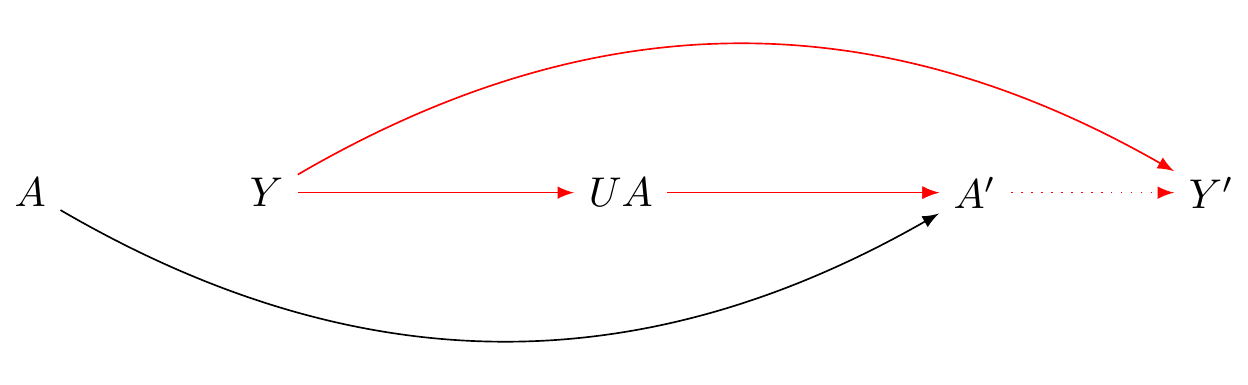
\includegraphics[width=1\textwidth,height=\textheight]{causal-diagrams-graph-abstract_files/figure-pdf/fig-dag-measure-selection-0-1.pdf}

}

\caption{\label{fig-dag-measure-selection-0}The figure illustrates the
bias arising measurement error of A' caused by Y. Although A and Y are
independent, their measured counterparts, A' and Y', are not. The
systematic error introduced by changes in Y opens a biasing path,
signified in red.}

\end{figure}%

\textbf{?@fig-dag-measure-selection} exposes the structure of bias where
post-outcome adjustment is necessary to mitigate or eliminate
measurement bias instigated by the outcome itself. Assume our interest
lies in quantifying the influence of belief in Big gods on social
complexity. We assumed that highly complex societies amend history,
eliminating traces of beliefs in lesser gods. If traces of beliefs in
lesser gods were recoverable through sources such as language, cultural
evolutoinary researchers would obtain better effect estimates.
\textbf{?@fig-dag-measure-selection} clarifies the intuition that
recovering echoes of the silenced is worthwhile for enhancing the
accuracy of our causal effect estimates.

\begin{figure}

\centering{

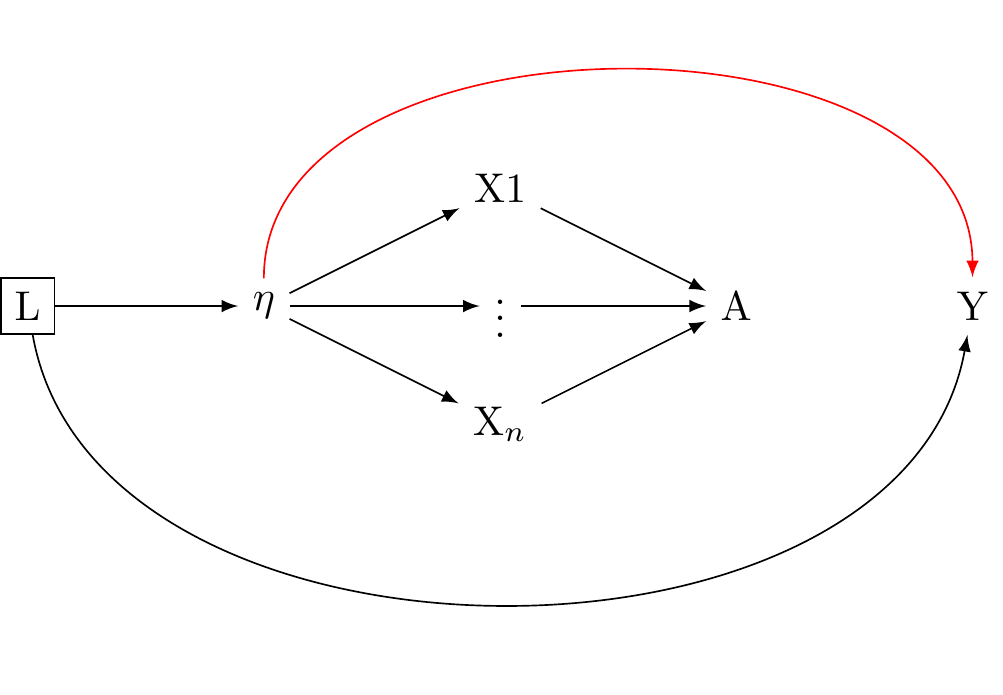
\includegraphics[width=0.8\textwidth,height=\textheight]{causal-diagrams-graph-abstract_files/figure-pdf/fig-structural-assumptions-reflective-model-1.pdf}

}

\caption{\label{fig-structural-assumptions-reflective-model}Structural
assumptions of the reflective model imply a univariate reality causes
the outcome. These assumptions are strong because they exclude
multivariate causes of the indicators for constructs, as well as
independent effects of the indicators on outcomes. Blue line indicates
assumed causal path. The figure is adapted from VanderWeele 2022.}

\end{figure}%

However, VanderWeele notes that the statistical model is consistent with
multiple causal models. The presumption that a univariate latent reality
underlies the reflective (and formative) latent factor models is a
stronger assumption than previously acknowledged. For example, an
alternative structural model equally compatible with the data is
presented in \textbf{?@fig-dag\_multivariate\_reality\_again}. Here,
multivariate reality gives rise to the indicators from which we draw our
measures. Indeed, for specific widely used measures, the assumption of a
univariate reality is so strong that they make testable assumptions.
VanderWeele and Vansteeland test the empirical examination assumptions
of widely used depression scales and find the assumptions fail
(\citeproc{ref-vanderweele2022b}{VanderWeele and Vansteelandt 2022}).
Although we cannot generally determine which structural models are
accurate, the data rule out the univariate model in the case that
VanderWeele and Vansteelandt (\citeproc{ref-vanderweele2022b}{2022})
examine.

\phantomsection\label{refs}
\begin{CSLReferences}{1}{0}
\bibitem[\citeproctext]{ref-vanderweele2022b}
VanderWeele, TJ, and Vansteelandt, S (2022) A statistical test to reject
the structural interpretation of a latent factor model. \emph{Journal of
the Royal Statistical Society Series B: Statistical Methodology},
\textbf{84}(5), 20322054.

\end{CSLReferences}



\end{document}
